\documentclass[a4paper]{report}

%====================== PACKAGES ======================

\usepackage[french]{babel}
\usepackage[utf8x]{inputenc}
%pour gérer les positionnement d'images
\usepackage{float}
\usepackage{amsmath}
\usepackage{graphicx}
\usepackage[colorinlistoftodos]{todonotes}
\usepackage{url}
%pour les informations sur un document compilé en PDF et les liens externes / internes
\usepackage{hyperref}
%pour la mise en page des tableaux
\usepackage{array}
\usepackage{tabularx}
%pour utiliser \floatbarrier
%\usepackage{placeins}
%\usepackage{floatrow}
%espacement entre les lignes
\usepackage{setspace}
%modifier la mise en page de l'abstract
\usepackage{abstract}
%police et mise en page (marges) du document
\usepackage[T1]{fontenc}
\usepackage[top=2cm, bottom=2cm, left=2cm, right=2cm]{geometry}
%Pour les galerie d'images
\usepackage{subfig}

%====================== INFORMATION ET REGLES ======================

%rajouter les numérotation pour les \paragraphe et \subparagraphe
\setcounter{secnumdepth}{4}
\setcounter{tocdepth}{4}

\hypersetup{							% Information sur le document
pdfauthor = {PALARD Nicolas}
pdftitle = {Stage Master 2 Informatique -
			RealityTech},			% Titre du document
pdfsubject = {Mémoire de Projet},		% Sujet
pdfkeywords = {Research, Augmented Reality, High performance},	% Mots-clefs
pdfstartview={FitH}}					% ajuste la page à la largueur de l'écran
%======================== DEBUT DU DOCUMENT ========================

\begin{document}

%régler l'espacement entre les lignes
\newcommand{\HRule}{\rule{\linewidth}{0.5mm}}

%page de garde
\begin{titlepage}
\begin{center}

% Upper part of the page. The '~' is needed because only works if a paragraph has started.

\includegraphics[width=0.35\textwidth]{./logos/ubx}~\\[1cm]

\textsc{\LARGE Université de Bordeaux - Reality Tech}\\[1.5cm]

\textsc{\Large }\\[0.5cm]

% Title
\HRule \\[0.4cm]

{\huge \bfseries Mémoire de stage\\
				Master 2 Informatique\\
				Image et son\\}

\HRule \\[1.5cm]

% Author and supervisor
\begin{minipage}{0.4\textwidth}
\begin{flushleft} \large
\emph{Auteur:}\\
Nicolas \textsc{PALARD}\\
\end{flushleft}
\end{minipage}
\begin{minipage}{0.4\textwidth}
\begin{flushright} \large
\emph{Client:} \\
Jérémy \textsc{Laviole}\\
\emph{Référent:} \\
Vincent \textsc{LEPETIT}
\end{flushright}
\end{minipage}

\vfill


\includegraphics[width=0.22\textwidth]{./logos/logo-rt-notext}~\\[1cm]
% Bottom of the page
{\large \today}

\end{center}
\end{titlepage}

%page blanche
\newpage
~
%ne pas numéroter cette page
\thispagestyle{empty}
\newpage

\renewcommand{\abstractnamefont}{\normalfont\Large\bfseries}
%\renewcommand{\abstracttextfont}{\normalfont\Huge}

\begin{abstract}
\hskip7mm

\begin{spacing}{1.3}

Dans le cadre de mon stage de fin d'étude, j'ai eu l'occasion de travailler chez \texttt{RealityTech}, une jeune startup dans le domaine de la réalité augmentée spatiale. Durant le temps que j'y ai passé, il m'a été demandé d'étudier les objectifs, les intérêts et les apports de cette technologie. J'ai tout d'abord pu l'apprivoiser par le biais de \texttt{PapARt}, le système de projection interactif que développe la société, avec lequel j'ai développé mes premières applications. Tout au long de ces développements, j'ai découvert les enjeux mais aussi les difficultés inhérentes à de tels systèmes. Ces diverses difficultés ainsi que la rigidité de \texttt{PapARt} m'ont amené à développer un prototype d'une nouvelle plateforme pour la société, dont le but était d'offrir de meilleures performances et d'être plus robuste que le système actuel, tout en en conservant les fonctionnalités. De l'optimisation matérielle à la refonte complète de l'architecture, en passant par l'optimisation algorithmique, il m'a été demandé d'opérer sur tous les fronts afin de créer un prototype viable. Un prototype n'allant pas sans tests, j'ai du m'atteler à réaliser une batterie de tests de performance qui ont permis de mettre en lumière les avancées mais aussi les défauts de ce dernier. Les performances n'étant pas le seul critère de validation du prototype, j'ai poursuivi mon stage en développant un module Unity permettant de le mettre à profit. En plus de permettre l'évaluation de l'utilisabilité du prototype, le module devait aussi fournir aux utilisateurs développeurs de \texttt{RealityTech} la possibilité de créer des applications de réalité augmentée spatiale en résolvant, pour ces derniers, les nombreuses problématiques liées au domaine. Ainsi, pour terminer mon stage, j'ai endossé le costume de l'utilisateur développeur et ai réalisé une application de démonstration en utilisant le module nouvellement créé afin d'en réaliser l'évaluation.\\

\textit{Mot-clés:} Réalité augmentée, réalité augmentée spatiale, interface tangible, programmation haute performance, microservices, unity, processing, vision par ordinateur.

\end{spacing}
\end{abstract}


\tableofcontents
\thispagestyle{empty}
\setcounter{page}{0}
%ne pas numéroter le sommaire

\newpage

%espacement entre les lignes d'un tableau
\renewcommand{\arraystretch}{1.5}

%====================== INCLUSION DES PARTIES ======================

~
\thispagestyle{empty}
%recommencer la numérotation des pages à "1"
\setcounter{page}{0}
\newpage

\chapter{Introduction}

Ce mémoire retracera les missions réalisées durant mon stage de Master 2 Informatique pour l'Image et le Son à l'Université de Bordeaux 1 effectué entre Avril et Septembre 2018 (6 mois) dans la société RealityTech. Ce rapport ne couvrira cependant que les 5 premiers mois du stage car la date de rendu de ce dernier précède d'un moi la date de fin du stage.

Le stage a donc été effectué chez RealityTech une jeune start-up de réalité augmentée spatiale. Issue de l'Inria de Bordeaux, l'institut national de la recherche en information et en automatique, cette dernière est la continuité d'un projet de recherche mené par Jérémy Laviole, ex ingénieur de recherche à l'Inria. PapARt\footnote{https://project.inria.fr/papart/fr/}. Paper Augmented Reality ToolKit est un kit de développement (SDK) permettant de créer des expériences de réalité augmentée sous forme d'applications de projection interactive dans des feuilles de papier. Les travaux actuellement effectués a RealityTech visent à améliorer et étendre ce système de projection. Le but est de pouvoir créer, via ce que propose la société, des expériences collaboratives où les objets physiques se mêlent parfaitement au monde numérique que ce soit en créant des interactions avec ceux ci, ou en leur rajoutant du contexte.

Actuellement, RealityTech se développe dans un incubateur de start-up appelé \texttt{La Banquiz}\footnote{http://labanquiz.com} situé 4 rue Eugène et Marc Dulout, a Pessac Centre. L'objectif de La Banquiz est de promouvoir des start-up Open Source\footnote{https://fr.wikipedia.org/wiki/Open\_source} et innovantes en leur apportant des formations, du coaching individuel et collectif, de l'aide pour la recherche de financement et tout ce qui gravite autour de l'accompagnement de jeunes entreprises.

A ce jour RealityTech ne travail qu'avec des laboratoire de recherche (comme ...) et cherche a étendre son secteur d'activité. Les systèmes proposés par la société fournissent les résultats espérés et la dynamique de celle ci s'oriente donc vers une commercialisation du produit. %Parler du fort besoin d'innovation logiciel (plateform haute performance, haut de gamme moyen de gamme bas de game. Expliquer le besoin de démo, de prototype, le salon qu'on a effecuté etc...
% Biblio : PapARt, Inria, Reality Tech, Realité Augmentée Spatiale

\section{Cadre et contexte}
\label{sec:contexte}
RealityTech fait actuellement partie de La Banquizz, un incubateur de startup situé a Pessac Centre.
% Expliquer le cadre de travail, incubateur, beaucoup de réunion, de démarchage, besoin d'applications de démonstration, besoin de prototype pour avoir des fonds etc autonomie très importante ..
% Parler du contexte  en terme de logiciel : volonté d'évolué et de partir vers une nouvelle base moins contraignante que celle présente actuellement + volonté d'ouverture au grand public (ce qui a fait que j'ai du dev unity) + modularité
% Peut être parler plus en détail de PapARt (calibration camera projecteur, expliqué qu'on travail avec des caméra, a l'échelle dans le monde réel (beaucoup de problèmes de calibration etc ...)

\begin{center}
Problématique du sujet
\end{center}


\section{Objectifs}
Le déroulement du stage a été fortement guidé par les besoins de la société.
\paragraph{Applications de démonstration}Le premier gros objectif du stage était le développement d'applications de démonstration en utilisant le produit de l'entreprise. Le but était de comprendre l'essence, le fonctionnement global du produit et ce qu'il était possible/impossible de réaliser avec celui ci. Cet objectif m'a permis d'acquérir à la fois une vision globale de l'architecture logiciel et du fonctionnement interne du kit de développement, et de l'architecture matérielle nécessaire a l'utilisation du kit. En développant ces applications de démonstration, j'ai acquis une vision globale du projet qui m'a permis d'avoir une certaine autonomie assez rapidement

\paragraph{Plateforme haute performance} Le deuxième objectif était de réaliser une preuve de concept haute performance du produit. En effet, comme je l'ai expliqué dans la partie sur le contexte (voir ~\ref{sec:contexte}), l'entreprise se lançait dans le développement d'une nouvelle plateforme haute performance.
% TODO pas fini

\paragraph{Kit de développement} Le dernière objectif était le développement d'un nouveau kit de développement pour Unity3D.  % TODO expliciter

\chapter{État de l'art}

Intro

\section{PapARt}

\section{Système de réalité augmentée spatiale}

\section{Bilan}
 
\chapter{Analyse des besoins}

Intro

\section{Besoins fonctionnels}

Après une analyse des besoins fonctionnels du projet, nous avons défini deux sous catégories. D'un côté, les besoins [...], de l'autre, les besoins [...].

\subsection{Sous-partie 1}

Bla

\subsection{Sous-partie 2}

Bla

\newpage

\section{Besoins non-fonctionnels}

Comme précédemment, nous avons choisi de distinguer deux catégories pour les besoins non-fonctionnels. D'une part, nous avons les besoins non-fonctionnels pour les [...], et d'autre part ceux pour [...]. Nous avons aussi pris en compte les contraintes de développement, que nous détaillerons à la fin de cette partie.

\subsection{Sous-partie 1}

Bla\\

Aperçu du rendu souhaité :

\begin{figure}[!h]
\begin{center}
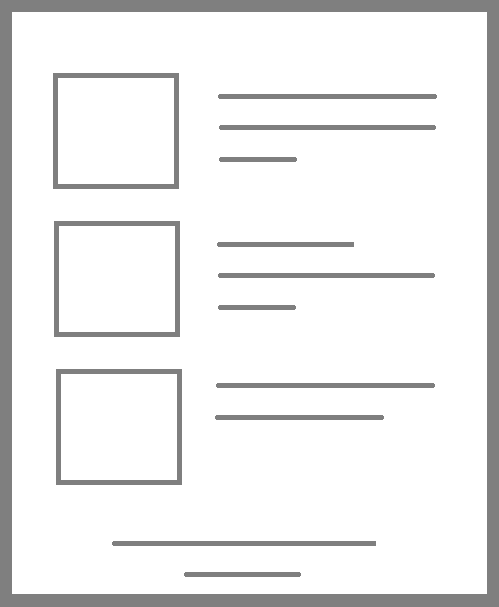
\includegraphics[height=10cm]{besoins/rendu}
\end{center}
\caption{Rendu attendu}
\end{figure}

\subsection{Sous-partie 2}

Bla

\newpage

\section{Développement}

Intro

\subsection{Tâches}

Bla\\


%tableau à taille fixée sur certaines colonnes (param sur la ligne \begin{tabularx}, voir wiki pour plus d'info sur la syntaxe
\begin{figure}[!h]
\begin{center}
\begin{tabularx}{17cm}{|c|p{6cm}|X|}
  \hline
  Priorité & Nom & Raison\\
  \hline
  1 & Tache 1 & Doit être vérifié en premier car sinon [...] \tabularnewline
  2 & Tache 2 & On doit pouvoir [...] \tabularnewline
  3 & Tache 3 & Comme les principales fonctionnalités permettant de tester sont opérationnelles, nous pouvons passer à cette tâche. \tabularnewline
  4 & Tache 4 & Parce que [...] \tabularnewline
  5 & Tache 5 & La tache 5 fait partie des principales [...]. \tabularnewline
  6 & Tache 6 & Dernière fonctionnalité essentielle à mettre en place. \tabularnewline
  7 & Tache 7 & Non-essentiel, mais apporterait un plus au projet. \tabularnewline
  8 & Tache 8 & Non-essentiel, mais apporterait un plus au projet. \tabularnewline
  \hline
\end{tabularx}
\end{center}
\caption{Tableau récapitulatif des tâches}
\end{figure}

\subsection{Tests}

Bla\\

\begin{figure}[!h]
\begin{center}
\begin{tabularx}{17cm}{|p{6cm}|X|}
  \hline
  Fonctionnalité & Test\\
  \hline
  Fonction 1 & Quand [...], vérifier [...]. \tabularnewline
  & Et quand [...], vérifier [...]. \tabularnewline
  Fonction 2 & Vérifier [...]. \tabularnewline
  Fonction 3 & Vérifier [...]. \tabularnewline
  Fonction 4 & Avoir [...]. \tabularnewline
  Fonction 5 & Accéder à [...]. \tabularnewline
   & Vérifier que [...]. \tabularnewline
  Fonction 6 & Accéder à [...]. \tabularnewline
   & Et vérifier [...]. \tabularnewline
  Fonction 7 & Installer [...]. \tabularnewline
   & Vérifier [...]. \tabularnewline
  Fonction 8 & Compter [...]. \tabularnewline
  \hline
\end{tabularx}
\end{center}
\caption{Tableau récapitulatif des tests}
\end{figure}

\chapter{Autre partie}

Dans cette partie nous cherchons à décrire dans un premier temps [...], puis, c[...].

\section{Partie 1}

Intro

\subsection{Sous-partie 1}

\begin{figure}[!ht]
\begin{center}

\includegraphics[height=12cm]{autre_partie/image1}
\end{center}
\caption[autre partie générale]{autre partie image 1\protect\footnotemark}
%\floatfoot{Source: (Citation command)}
% avec le package "floatrow"
\end{figure}

%footnote protected pour apparaitre dans la légende d'une image
\footnotetext{Schéma d'après : \textit{Auteur 1 \& Propriétaire image}, LICENCE (cf. ref. \cite{cite4})}

\newpage{}

\subsection{Sous-partie 2}

\begin{figure}[!ht]
\begin{center}

\includegraphics[height=12cm]{autre_partie/image2}
\end{center}
\caption[autre partie]{autre partie globale de notre quelque chose}
\end{figure}

Nous retrouvons ici, blabla\footnote{Application bla - Interface blabla} [...].

\subsubsection{Sous-sous-partie 1}

Le bla (cf. ref. \cite{cite6}) est [...]:

\begin{itemize}
\item item1;
\item item2;
\item item3;
\item item4;
\item item5.
\end{itemize}

\newpage

\subsubsection{Sous-sous-partie 2}

%Les lignes :
% \setcounter{secnumdepth}{4}
% \setcounter{tocdepth}{4}
%dans le fichier "main.tex" permettent de faire en sorte que les paragraphes soient interprété comme des titres de niveau 5
\paragraph{Paragraphe 1 (agissant comme titre niveau 5)}
%forcer un saut de ligne
~\\
\hskip7mm

\begin{figure}[!ht]
\begin{center}

\includegraphics[height=6cm]{autre_partie/image3}
\end{center}
\caption[Structure d'unz autre chose]{Structure d'une autre chose\protect\footnotemark}
\end{figure}

Ce schéma représente bla.

\footnotetext{Schéma et explication d'après le wiki bla (cf. ref. \cite{cite0})}

\paragraph{Paragraphe 2}
~\\
\hskip7mm

%fixer les floats précédemment définis
%\FloatBarrier

Bla

\subparagraph{Sous-paragraphe 1}
~\\
\hskip7mm

Bla

\begin{figure}[H]
\begin{center}

\includegraphics[height=10cm]{autre_partie/image4}
\end{center}
\caption{Diagramme de truc}
\end{figure}

\subparagraph{Sous-paragraphe 2}
~\\
\hskip7mm

Bla\\

Bla

\subparagraph{Sous-paragraphe 3}
~\\
\hskip7mm

Bla

\subsubsection{Sous-sous-partie 3}

Bla

\section{Partie 2}

Bla

\footnotetext{D'après le schéma disponible sur la documentfation officielle disponible sur le site blalbla}

Bla

\subsection{Sous-partie 1}

Bla

\subsection{Sous-partie 2}

Bla

\paragraph*{Paragraphe 1 (n'apparaitra pas dans l'index)}
Bla

\paragraph*{Paragraphe 2}
Bla

\paragraph*{Paragraphe 3}
Bla

\subsection{Sous-partie 3}

Bla

\chapter{Résultats}

\section{Partie 1}

Intro

\subsection{Sous-partie 1}

\paragraph*{Paragraphe 1 (n'apparaitra pas dans l'index)} Bla

\paragraph*{Paragraphe 2} Bla

\paragraph*{Paragraphe 3} Bla

\subsection{Sous-partie 2}

Bla

\subsection{Sous-partie 3}

Bla

\section{Partie 2}

Intro

\subsection*{Sous-partie 1 ('apparaitra pas dans l'index)} Bla

\paragraph*{Paragraphe 1 ('apparaitra pas dans l'index)} Bla

\paragraph*{Paragraphe 2} Bla

\paragraph*{Paragraphe 3} Bla

\newpage

\subsection*{Sous-partie 2}

Bla

%galerie d'image
\begin{figure}[htp]
  \centering
  \subfloat[Première image]{\label{fig:première}
\includegraphics[scale=0.8]{resultats/gallerie}}
  ~ %espace entre deux images sur une même ligne
  \subfloat[Deuxième image]{\label{fig:deuxième}
\includegraphics[scale=0.8]{resultats/gallerie}}
  ~
  \subfloat[Troisième image]{\label{fig:troisième}
\includegraphics[scale=0.8]{resultats/gallerie}}
  ~\\ %saute une ligne dans la galerie d'image
  \subfloat[Quatrième image]{\label{fig:quatrième}
\includegraphics[scale=0.8]{resultats/gallerie}}
  ~
  \subfloat[Cinquième image]{\label{fig:cinquième}
\includegraphics[scale=0.8]{resultats/gallerie}}
  \caption{Différents screenshots quelque chose, en gallerie}
  \label{fig:gallerie1}
\end{figure}

\chapter{Bilan}

%Rappel du context
Intro / Rappel Contexte

Nous avons donc pu en tirer la problématique suivante :

\begin{center}
\hskip7mm
Problématique du sujet
\end{center}

Bla

Bla\\

Bla\\

%Rappel des résultats
Bla

Bla\\

Bla

Bla

\newpage

%Conclusion/Perspectives
Bla

Bla\\

Bla

%Ne pas numéroter cette partie
\part*{Annexes}
%Rajouter la ligne "Annexes" dans le sommaire
\addcontentsline{toc}{part}{Annexes}

\chapter*{Annexe 1}
\addcontentsline{toc}{chapter}{Annexe 1}

%changer le format des sections, subsections pour apparaittre sans le num de chapitre
\makeatletter
\renewcommand{\thesection}{\@arabic\c@section}
\makeatother

%recommencer la numérotation des section à "1"
\setcounter{section}{0}

Intro

\section{Partie 1}

Bla

\subsection{Sous-partie 1}

Bla

\subsection{Sous-partie 2}

Bla

\subsection{Sous-partie 3}

Bla

\section{Partie 2}

Bla

\subsection{Sous-partie 1}

Bla

\subsection{Sous-partie 2}

Bla

\subsection{Sous-partie 3}

Bla

\chapter*{Annexe 2}
\addcontentsline{toc}{chapter}{Annexe 2}

%recommencer la numérotation des section à "1"
\setcounter{section}{0}

Intro

\section*{Prérequis}
\addcontentsline{toc}{section}{Prérequis}

Bla

\begin{itemize}
\item item1;
\item item2;
\item item3;
\item item4.
\end{itemize}

Bla

\section{Partie 1}

Bla

\subsection{Sous-parie 1}

Bla

\subsection{Sous-parie 2}

Bla

\section{Partie 2}

\begin{center}
\textsc{Attention !}

\textit{Texte d'avertissement}
\end{center}

Bla

\newpage

\section{Partie 3}

Bla

\begin{figure}[!ht]
\begin{center}
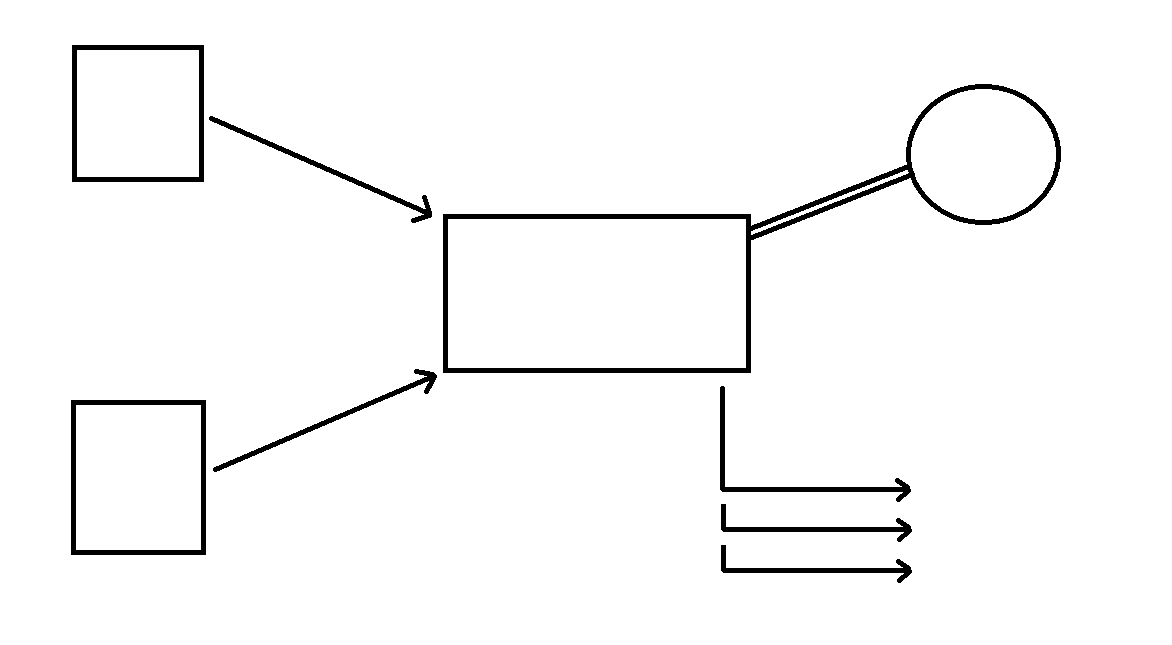
\includegraphics[height=8cm]{presentation/schema}
\end{center}
\caption[schema]{Presentation schema}
\end{figure}

\paragraph*{Paragraphe 1}
~\\
\hskip7mm

Bla

\paragraph*{Paragraphe 2}
~\\
\hskip7mm

Bla

\paragraph*{Paragraphe 3}
~\\
\hskip7mm

Bla

\chapter*{Annexe 3 - Unity diagramme d'exécution des fonctions}
\addcontentsline{toc}{chapter}{Annexe 3 - Unity diagramme d'exécution des fonctions}
\label{annexe:unity}

\begin{figure}
\centering
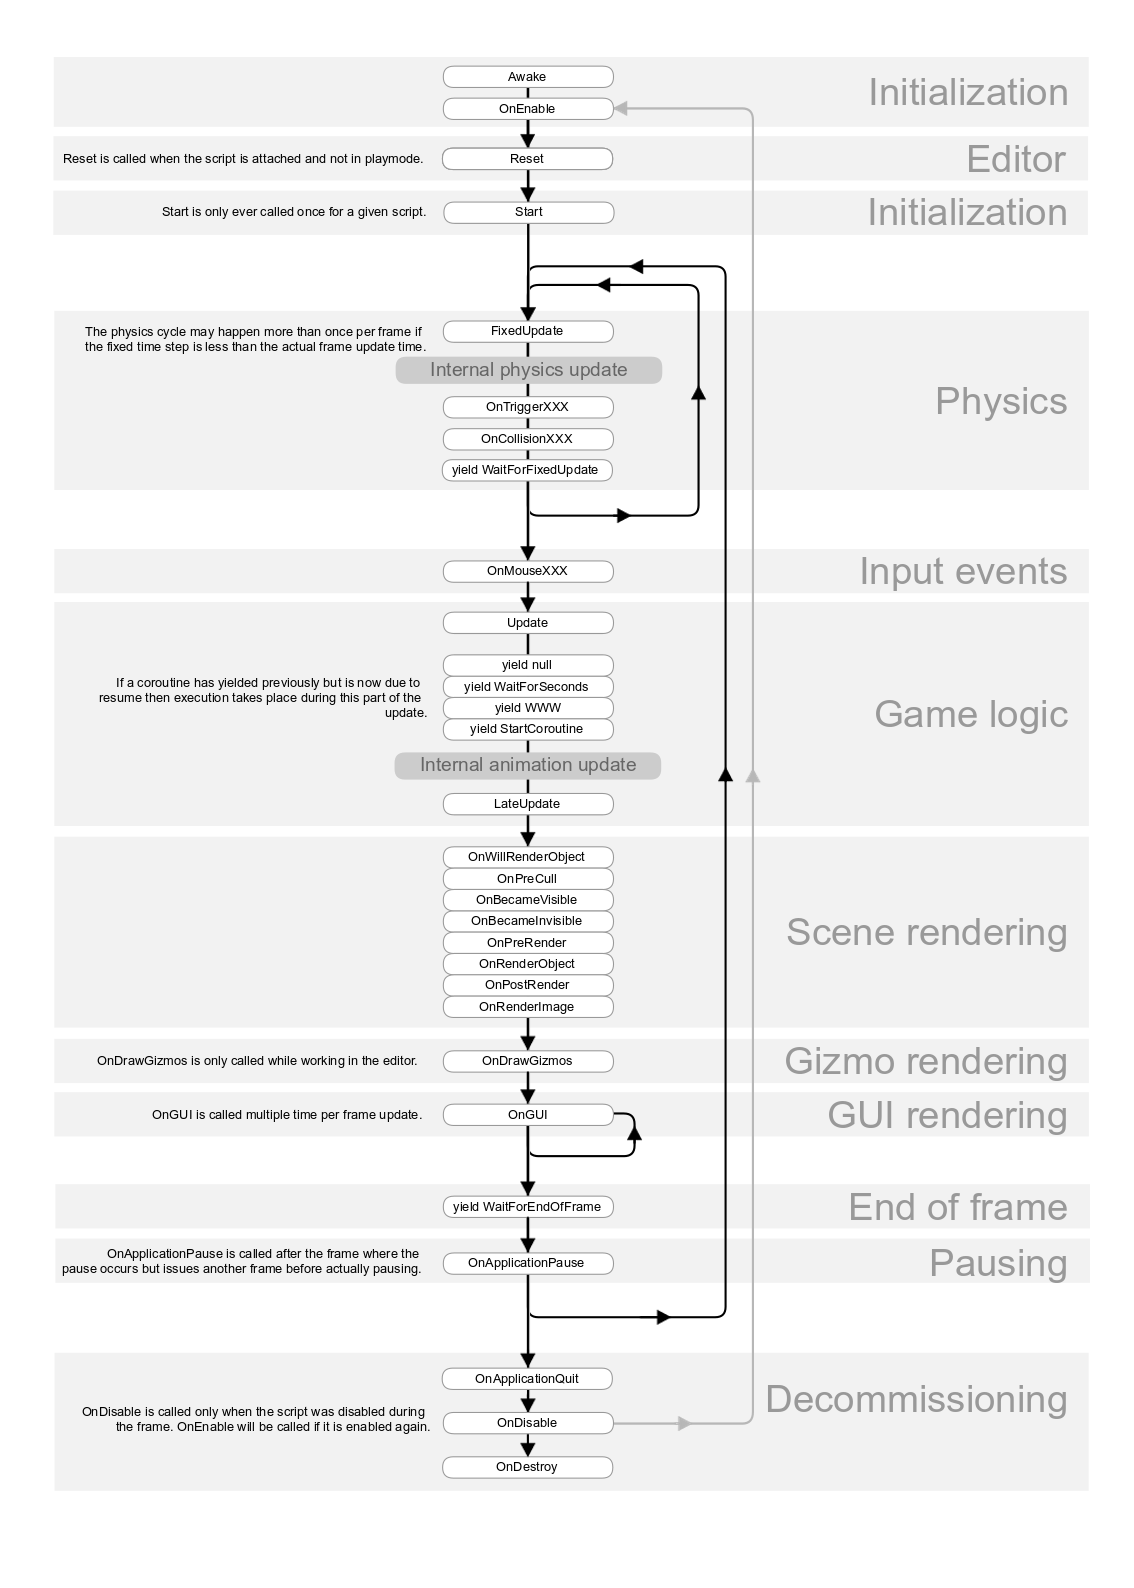
\includegraphics[width=\linewidth]{images/monobehaviour_flowchart}
\end{figure}

\newpage

%récupérer les citation avec "/footnotemark"
\nocite{*}

%choix du style de la biblio
\bibliographystyle{plain}
%inclusion de la biblio
\bibliography{bibliographie.bib}
%voir wiki pour plus d'information sur la syntaxe des entrées d'une bibliographie

\end{document}